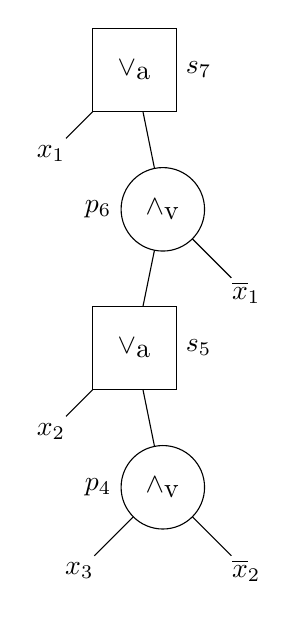
\begin{tikzpicture}
\definecolor{neutralcolor}{RGB}{0,0,0}
\definecolor{pathcolor}{RGB}{0,0,0}
\definecolor{fillcolor}{RGB}{255,255,255}
\definecolor{background}{RGB}{225,225,225}
\definecolor{highcolor}{RGB}{0,0,0}
\definecolor{lowcolor}{RGB}{0,0,0}
\draw (1.32,6.62) [thin,neutralcolor] -- (0.26,5.56);
\draw (1.32,6.62) [thin,neutralcolor] -- (1.68,4.85);
\draw (1.68,4.85) [thin,neutralcolor] -- (2.74,3.79);
\draw (1.68,4.85) [thin,neutralcolor] -- (1.32,3.09);
\draw (1.32,3.09) [thin,neutralcolor] -- (0.26,2.03);
\draw (1.32,3.09) [thin,neutralcolor] -- (1.68,1.32);
\draw (1.68,1.32) [thin,neutralcolor] -- (2.74,0.26);
\draw (1.68,1.32) [thin,neutralcolor] -- (0.62,0.26);
\draw [thin,fill=fillcolor,draw=neutralcolor] (1.68,4.85) circle [radius=0.53];
\node at (1.68,4.85) {$\mathbin{\land_{\textrm{v}}}$};
\draw [thin,fill=fillcolor,draw=neutralcolor] (1.68,1.32) circle [radius=0.53];
\node at (1.68,1.32) {$\mathbin{\land_{\textrm{v}}}$};
\draw [thin,fill=fillcolor,draw=fillcolor] (2.74,0.26) circle [radius=0.26];
\node at (2.74,0.26) {$\overline{x}_2$};
\draw [thin,fill=fillcolor,draw=neutralcolor] (0.79,6.09) rectangle (1.85,7.15);
\node at (1.32,6.62) {$\mathbin{\lor_{\textrm{a}}}$};
\draw [thin,fill=fillcolor,draw=neutralcolor] (0.79,2.56) rectangle (1.85,3.62);
\node at (1.32,3.09) {$\mathbin{\lor_{\textrm{a}}}$};
\draw [thin,fill=fillcolor,draw=fillcolor] (2.74,3.79) circle [radius=0.26];
\node at (2.74,3.79) {$\overline{x}_1$};
\draw [thin,fill=fillcolor,draw=fillcolor] (0.26,2.03) circle [radius=0.26];
\node at (0.26,2.03) {$x_2$};
\draw [thin,fill=fillcolor,draw=fillcolor] (0.62,0.26) circle [radius=0.26];
\node at (0.62,0.26) {$x_3$};
\draw [thin,fill=fillcolor,draw=fillcolor] (0.26,5.56) circle [radius=0.26];
\node at (0.26,5.56) {$x_1$};
\node [right] at (1.85,6.62) {$s_7$};
\node [left] at (1.15,4.85) {$p_6$};
\node [right] at (1.85,3.09) {$s_5$};
\node [left] at (1.15,1.32) {$p_4$};
\end{tikzpicture}%%
